\chapter{Einleitung \label{chap_einleitung}}
Das immer höher werdende Verkehrsaufkommen stellt die Infrastruktur vor immer größere Herausforderungen. Neben der Vermeidung von Staus darf die Vermeidung von Verletzten und Toten durch Kraftfahrzeug Verkehr nicht aus dem Fokus verloren werden. Bei der Vermeidung von Verletzten und Toten wurden in den letzten Jahren große Fortschritte erzielt. So haben passive Systeme, wie beispielsweise Anschnallgurte oder Airbags, bereits viele Menschenleben gerettet. Ein andere Möglichkeit zum Erreichen dieses Ziels ist die Steigerung der aktiven Sicherheit. Es ist sinnvoller einen Unfall zu verhindern, als dessen Folgen durch passive Sicherheitselemente im Fahrzeug abzumildern. Besonders im Hinblick auf den Fußgängerschutz spielt eine aktive Technik ihre Vorteile aus, da sich Fußgänger nicht durch Knautschzonen oder Airbags schützen können. Hier gilt es besonders, Unfälle zu vermeiden.

Ein Lösungsansatz für diese Probleme ist, dass die Kommunikation zwischen Verkehrsteilnehmern ermöglicht wird. Eine Kommunikation zwischen den Teilnehmern ermöglicht beispielsweise ein \glqq Sehen um die Ecke\grqq. Das \glqq Sehen um die Ecke\grqq~ermöglicht es, dass der Fahrer vor Ereignissen oder Hindernissen gewarnt wird, bevor er sie sehen kann. Solche Ereignisse können ein Stauende hinter einer Kurve oder ein Fußgänger auf der Straße sein. Aber auch vor Falschfahrern kann effektiv gewarnt werden, wenn hierfür eine Kommunikationsmöglichkeit besteht.

Auch die Effizienz der Verkehrsinfrastruktur kann durch eine Kommunikation zwischen Verkehrsteilnehmern erhöht werden. Dadurch kann bei den Verkehrsteilnehmern auch viel Frust, der beispielsweise durch verstopfte Straßen oder nicht angepasste Verkehrsregelungen entsteht, vermieden werden. Da die regulierenden Elemente der Verkehrsinfrastruktur auf aktuelle Ereignisse reagieren müssen, muss neben der Kommunikation zwischen den Fahrzeugen auch eine Kommunikation zwischen Fahrzeugen und Infrastruktur sicher gestellt werden.

Diese Aufgaben werden durch eine \ac{C2C}, oder allgemeiner gesagt, durch eine \ac{C2X} sichergestellt. 

\section{ETSI ITS}
Im europäischen Bereich wird das System \ac{ITS} genannt und von dem \ac{ETSI} standardisiert. Dabei handelt es sich um gesamtes Kommunikationssystem mit eigenem Protokollstack. 

\begin{figure}[h]
	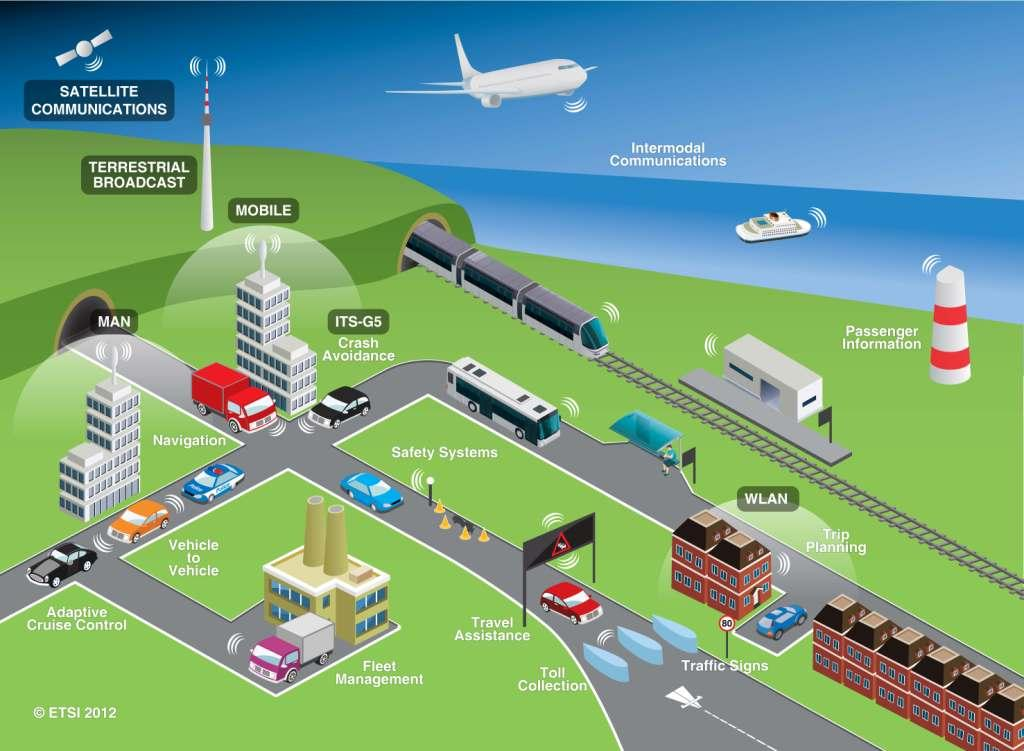
\includegraphics[width=0.95\textwidth]{content/images/00_einleitung/ETSI_ITS_09_2012.jpg}
	\caption{Übersicht über ITS \cite{ITS_vorstellung}}
	\label{fig:itsVorstellung}
\end{figure}

Die \autoref{fig:itsVorstellung} gibt einen Überblick über die Möglichkeiten von \ac{ITS} dabei ist leicht zu erkennen, dass \ac{ITS} über die reine \ac{C2C} Kommunikation hinaus geht. Das System bietet die Grundlage für verschiedene Anwendungsfälle. Sie können die verschiedensten Ziele verfolgen. So sind beispielsweise neben der Erhöhung der Sicherheit oder der Verkehrseffizienz auch Anwendungsfälle möglich, die dem Komfort der Verkehrsteilnehmer dienen. All diesen Anwendungen wird eine Plattform geboten, die die Zuverlässigkeit des Systems und die Sicherheit der Teilnehmer sicherstellt. So muss sich der Entwickler einer solchen Anwendung keine Gedanken um den Datenschutz machen, da dieser bereits durch \ac{ITS} sichergestellt wird.

Die folgende Ausarbeitung soll dem Leser das \ac{ETSI} \ac{ITS} System näher bringen und ihm einen Überblick über den Aufbau, die Funktion und die Leistungsfähigkeit vermitteln. Bei der Entstehung der Ausarbeitung sind die Forschungsgruppen und Konsortien nicht berücksichtigt worden, obwohl ein Großteil der Arbeit dort erledigt wurde und wird. Die Ausarbeitung bezieht sich lediglich auf die Standards, die vom \ac{ETSI} veröffentlich wurden. Einige der Konzepte muten abstrakt an. Sie werden erst bei der Implementierung durch die \ac{OEM} oder Forschungsgruppen konkret.

\section{Begriff Car to Car}
Der Begriff \ac{C2C} beschreibt die reine Kommunikation zwischen \ac{ITS} fähigen Fahrzeugen. Dabei wird die Luftschnittstelle und die eigens hierfür entwickelte \ac{ITS} Architektur genutzt. Da diese Architektur als Gesamtes betrachtet werden muss, wird in der Ausarbeitung das gesamte \ac{ETSI} \ac{ITS} System beschrieben.  



\section{Beteiligte Konsortien}
\todo{EVtl. noch Konsortien aufzählen}

